\documentclass[oneside,brazil,a4paper]{normas-utf-tex}


\usepackage[utf8]{inputenc}
\usepackage{fontenc}
\usepackage{babel}

\usepackage{url}

\usepackage[alf,abnt-emphasize=bf,bibjustif,recuo=0cm, abnt-etal-cite=2, abnt-etal-list=99]{abntcite}

\usepackage{graphicx}

\usepackage[final]{pdfpages}

% desativa hifenizacao mantendo o texto justificado.
% thanks to Emilio C. G. Wille
% \tolerance=1
% \emergencystretch=\maxdimen
% \hyphenpenalty=10000
% \hbadness=10000

\sloppy

\usepackage{subfig}
\usepackage{multirow}
\usepackage{array}
\usepackage{tabularx}
\newcommand{\fullcell}{\multicolumn{1}{>{\columncolor[gray]{0.5}}c}{}}
\newcommand{\fullcellline}{\multicolumn{1}{>{\columncolor[gray]{0.5}}c|}{}}
\newcommand{\mc}[3]{\multicolumn{#1}{#2}{#3}}
\newcommand{\y}{\rule{8pt}{4pt}}
\newcommand{\n}{\hspace*{8pt}}

\instituicao{Universidade Tecnológica Federal do Paraná}
\programa{Curso Superior de Tecnologia em Sistemas para Internet}
\area{Tecnologia em Sistemas para Internet}

\documento{Trabalho de Conclusão de Curso}
\nivel{Graduação}
\titulacao{Tecnólogo}

\titulo{Recomendação de especialistas para novatos em projetos de software livre baseada em suas contribuições} 
\title{\MakeUppercase{Identification of experts to newcomers in open source projects based upon their contributions}} % titulo do trabalho em ingles
\autor{Erick William dos Santos} % autor do trabalho
\cita{SANTOS, Erick William} % sobrenome (maiusculas), nome do autor do trabalho
\palavraschave{novato, especialista, sistema de recomendação, software livre} % palavras-chave do trabalho
\keywords{newcomer, expert, recommender system, open source software} % palavras-chave do trabalho em ingles

\comentario{\hyphenpenalty=10000\UTFPRdocumentodata\ apresentado ao \UTFPRprogramadata\ da \ABNTinstituicaodata\ como requisito parcial para obtenção do grau de \UTFPRtitulacaodata\ em \UTFPRareadata.}

\orientador{Dr. Marco Aurélio Graciotto Silva}
\coorientador[Coorientador:]{Me. Igor Fábio Steinmacher}
%\orientador[Orientadora:]{Nome da Orientadora} % <- no caso de orientadora, usar esta sintaxe


\local{Campo Mourão - PR} % cidade
\data{\the\year} % ano automatico


\usepackage[capitalise]{cleveref}
\crefname{chapter}{Cap\'itulo}{Cap\'itulos}
\Crefname{chapter}{Cap\'itulo}{Cap\'itulos}
\crefname{section}{Se\c{c}\~ao}{Se\c{c}\~oes}
\Crefname{section}{Se\c{c}\~ao}{Se\c{c}\~oes}
\crefname{line}{Linha}{Linhas}
\Crefname{line}{Linha}{Linhas}
\crefname{table}{Tabela}{Tabelas}
\Crefname{table}{Tabela}{Tabelas}
\crefname{figure}{Figura}{Figuras}
\crefname{figure}{Figura}{Figuras}
\Crefname{figure}{Figura}{Figuras}
\crefname{subfigure}{Figura}{Figuras}
\Crefname{subfigure}{Figura}{Figuras}
\crefname{equation}{Equa\c{c}\~ao}{Equa\c{c}\~oes}
\Crefname{equation}{Equa\c{c}\~ao}{Equa\c{c}\~oes}
\crefname{lstlisting}{C\'odigo-fonte}{C\'odigos-fonte}
\Crefname{lstlisting}{C\'odigo-fonte}{C\'odigos-fonte}
\crefname{lstnumber}{Linha}{Linhas}
\Crefname{lstnumber}{Linha}{Linhas}
\crefrangelabelformat{chapter}{#3#1#4~a~#5#2#6}
\crefrangelabelformat{section}{#3#1#4~a~#5#2#6}

\sloppy


\begin{document}

\capa
\folhaderosto

% TODO: aproveite aqui para agradecer as pessoas que colaboraram, de alguma forma, com sua graduação
\begin{agradecimentos}
Quero agradecer, em primeiro lugar, aos meus pais Judite Emidia dos Santos e Gabriel Silva Santos por todo apoio e incentivo durante todo o curso. A todos os professores da Coordenação de Informática da UTFPR, por todos esses anos transmitindo um conhecimento seguro e paciente. Em especial aos professores Marco Aurélio Graciotto Silva e Igor Steimacher, pelo incentivo à execução deste trabalho.
\end{agradecimentos}

% TODO: atualizar com resultados
\begin{resumo}
Para o sucesso de um projeto de software livre, é necessária a participação de colaboradores. No entanto, eles exercem as atividades em caráter voluntário e o seu vínculo não é regido por regras trabalhistas, mas no retorno pessoal que obtém das interações no projeto. Em especial quanto aos novos colaboradores, é de particular importância que sejam recebidos de forma correta pela comunidade que desenvolve o software. Neste trabalho foi desenvolvido um mecanismo de seleção para encontrar desenvolvedores do projeto que possam ser indicados para auxiliar e orientar estes novos contribuintes. Como resultado desta abordagem, foi implantado um mecanismos de recomendação de especialistas aplicando aspectos temporais para contribuir com o sucesso do projeto e  melhorar a comunicação dos novatos com os demais desenvolvedores.
\end{resumo}

% TODO: atualizar com resultados
%
\begin{abstract}
Open source software projects require the participation of collaborators in order to achieve success. However, such collaborators work on a voluntary basis, without a formal association with the project, based only on personal and community interests. For new developers -- newcomers --, it is particulary important the reception of the community that drives the project. In this work, a recommendation mechanism has been developed to select experienced developers to mentor newcomers. The conceived algorithm considered temporal aspects, aiming at reducing the withdraw ratio of newcomers due to lack of support or initial mentoring in the project.
\end{abstract}


\listadefiguras
\clearpage
\listadetabelas
\sumario



\chapter{Introdução}
\label{cap:intro}
  
A busca por software livre (OSS) aumentou muito: não só usuários, mas grandes empresas já adotam esta prática. O software livre conseguiu esta popularidade pela qualidade do produto (software) e por ter a característica de compartilhar não apenas seu produto final, mas os demais artefatos de engenharia, a destacar o seu código fonte. Graças a este compartilhamento novas aplicações podem ser desenvolvidas sem ter que partir do zero. Portanto, tem tido um impacto duradouro sobre a forma como o software é desenvolvido, divulgado e adaptado.

Uma característica importante de projetos de software livre é a comunidade que o desenvolve, constituída significativamente por voluntários: desenvolvedores que participam livremente dos projetos que consideram atraentes~\cite{Madey-etal:2002}. De fato, o sucesso de um projeto de software livre é improvável sem uma comunidade que forneça uma plataforma para que desenvolvedores e usuários colaborem uns com os outros~\cite{YeKishida-etal:2003}. 

O desenvolvimento em comunidade de software possui alguns desafios inerentes a esse aspecto colaborativo. Por exemplo, a falta de conhecimento do próprio software poderia afetar negativamente a produtividade da equipe. Esse problema é claramente percebido sempre que um usuário precisa da ajuda de alguém ainda desconhecido e localizado remotamente, porque a comunicação síncrona com os membros da equipe, em grande parte das vezes, é muito restrita~\cite{Moraes-etal:2010}. Tais limitações atrasam o desenvolvimento do processo de colaboração entre os membros da equipe. 

Uma pergunta que surge com frequência dentro do contexto de tais projetos é ``quem deve trabalhar ou contribuir nesta tarefa?''. Abordagens para identificar e recomendar desenvolvedores, utilizando técnicas de aprendizagem de máquina e análise de redes sociais~\cite{Naguib-etal:2013}, podem auxiliar na indicação desses especialistas, de modo que o desenvolvedor mais adequado pode ser encontrado para ajudar a realizar uma dada tarefa~\cite{Robbes-etal:2013} e contribuir para uma colaboração mais efetiva entre os desenvolvedores. Por exemplo, considere um dúvida sobre o componente de impressão de uma aplicação. Tal componente está relacionado com vários arquivos de código fonte, os quais estão armazenados em um sistema de controle de versão (repositório). Os desenvolvedores que fizeram alterações em tais arquivos, supostamente, possuem domínio sobre a implementação das funcionalidades de impressão e, portanto, poderiam ser considerados especialistas. Assim, uma boa recomendação de especialistas seria selecionar e indicar aqueles desenvolvedores que fizeram mais alterações nos arquivos em questão.

Mecanismos de recomendação de especialistas são particularmente úteis para os voluntários ingressantes no projeto, doravante denominados novatos. Dada a experiência inexistente no projeto OSS em que ingressa, eles não conhecem os demais participantes da comunidade e, geralmente, não possuem conhecimento suficiente sobre o domínio do software a ponto de iniciar as contribuições. Em face a essas dificuldades, muitos novatos desistem de contribuir. Não obstante, também sabemos que o ingresso e a retenção de novatos é importante para o sucesso dos projetos~\cite{Yunrim-etal:2009}. 

Dessa forma, a implantação de mecanismos de recomendação de especialistas pode contribuir para o sucesso do projeto ao manter os novatos e melhorar a comunicação desses com os demais desenvolvedores~\cite{Steinmacher-etal:2012} Por exemplo, para tratar essa questão pode-se recomendar um especialista (mentor) para orientar e auxiliar tal novato nas primeiras interações no projeto, servindo como um instrumento para melhorar a retenção. Enquanto isso, do ponto de vista do novato, tais mecanismos de recomendação auxiliam na inserção do projeto e reduzem a frustração de interações infrutíferas, que será auxiliado em sua participação no projeto e no desenvolvimento de competências e habilidades.

O objetivo deste trabalho é implementar um mecanismo de recomendação de especialistas para novatos baseado em dados contidos em projetos de software livre, tais como repositórios de código fonte, lista de discussões e gerenciadores de tarefa. Especificamente, as metas são:

\begin{itemize}
    \item identificar dados disponíveis e características a serem extraídas dos artefatos de software disponíveis,

    \item implementar um algoritmo de recomendação que considere a questão temporal, tal como apresentado na literatura em trabalhos como, por exemplo, o de ~\citeonline{Robbes-etal:2013},

    \item alterar o algoritmo implementado para considerar informações relevantes à recomendações feitas para novatos,
    
    \item avaliar os resultados obtidos com os algoritmos implementados.
\end{itemize}

A partir do estudo sobre as disciplinas de mineração de repositório de software e recomendação de sistemas, foram identificados dados e estratégias tipicamente utilizados para a recomendação de especialistas em projetos de software livre, tal como exposto no \cref{cap:teoria}. Posteriormente, de acordo com o método de pesquisa descrito no \cref{cap:metodo}, escolheu-se um algoritmo para recomendação e a alteração para considerar aspectos  para favorecer a recomendação de mentores e implementou-se uma ferramenta para a mineração de projetos de software e recomendar mentores. Dois algoritmos foram propostos: com e sem decaimento para analisar a  contribuição para definição da experiencia do desenvolvedor. Para este estudo, analisou-se o projeto LibreOffice. 

Os algoritmos, a ferramenta e a análise do projeto estão descritos no \cref{cap:resultados}. Foram analisados novatos com significativa participação na comunidade no período de seis meses a partir da sua entrada. Em relação aos novatos mais ativos, ambos os algoritmos de recomendação, com e sem decaimento, obtiveram resultados satisfatórios quando comparados com os desenvolvedores experientes que atenderam aos novatos. Observou-se ainda que a recomendação com decaimento possui melhor precisão para novatos com mais interações sociais. No entanto, ao analisar os novatos menos ativos, ambas não obtiveram sucesso em suas recomendações, apresentando desenvolvedores experientes, porém não os desenvolvedores que efetivamente interagiram com estes novatos.



\chapter{Referencial teórico}
\label{cap:teoria}

\section{Delimitação do tema}
\label{sect:tema}

Com o objetivo de entender e levantar diversos problemas sobre recomendação de especialistas para novatos, é necessário analisar técnicas para o desenvolvimento de sistemas de recomendação voltados para o domínio de engenharia de software. No âmbito desta proposta, estudaram-se fundamentos e trabalhos sobre mineração de repositórios de software, que trata da extração de informações a partir de repositórios de software, as quais subsidiam a implementação de sistemas de recomendação. 


\subsection{Mineração de repositórios de software}

Mineração de Dados (do inglês \textit{Data Mining}) está se tornando cada vez mais popular entre os desenvolvedores como uma ferramenta de descoberta de informações~\cite{Cortes-etal:2002}. Atividades de mineração de dados referem-se à extração de conhecimento útil e previamente desconhecido de grandes quantidades dados e de diversos formatos, por meio da aplicação de algoritmos que extraem modelos e padrões representativos, obtendo-se informações que podem ser utilizadas para guiar decisões em condições de certeza limitada~\cite{Fayyad-etal:1996}.

Uma das variantes desta mineração chama-se mineração de repositórios de software (MSR, do inglês \textit{Mining Software Repositories}). MSR tem como principal alvo os dados relacionados ao processo de desenvolvimento de software, tais como listas de discussões, código fonte, fóruns, gerenciamento de tarefas e controladores de versão~\cite{Bird-etal:2006}. A prática de minerar dados tem se apresentado como uma abordagem importante para descoberta de novos padrões e tendências de desenvolvimentos, que são imperceptíveis em nível de código, mas não ao se observar os demais artefatos de engenharia de software.

A execução da mineração de repositórios de software é organizada em três etapas, tal como apresentado na \cref{fig:mine}, integrando-se funcionalidades, técnicas e algoritmos, visando esclarecer a interatividade do objetivo da mineração de dados com as técnicas a serem empregadas~\cite{Xie-etal:2009, Cortes-etal:2002}. A primeira etapa abrange a identificação e obtenção dos dados.  Os dados podem ser obtidos através dos repositórios onde se encontram o código fonte, histórico de mudanças e demais artefatos de engenharia de software, mostrados na base da \cref{fig:mine}.

\begin{figure}[hbt]
        \centering
        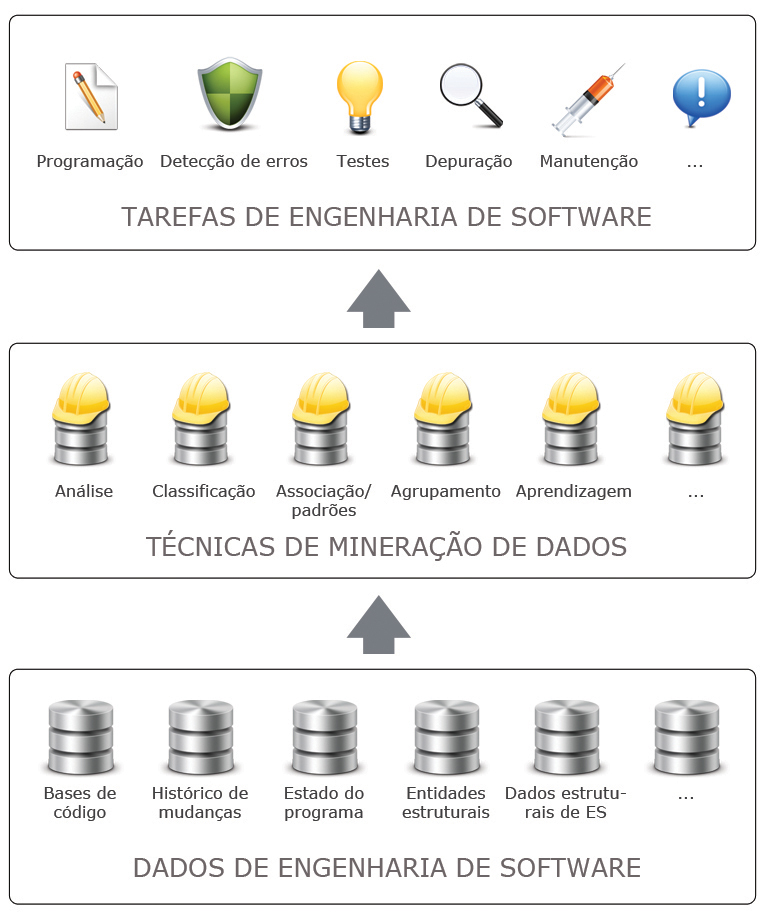
\includegraphics[width= .8\textwidth]{figuras/mineracao}
        \caption[Etapas da mineração de repositórios de software.]{Etapas da mineração de repositórios de software~\cite{Cortes-etal:2002}.}
        \label{fig:mine}
\end{figure}

A segunda tapa consiste em utilizar as técnicas de mineração de dados e trabalhar as informações armazenadas. Aplicando técnicas de classificação, agrupamento de informações relevantes, aprendizagem de máquina, dentre outras, é possível obter resultados e comportamentos relevantes para compreender o desenvolvimento de software e a execução das tarefas associadas. A terceira e última etapa trata da utilização das informações obtidas durante a análise para auxiliar a execução das atividades de engenharia de software. Por exemplo, aplicar práticas para melhorar as estruturas e métodos de programação, incentivar a execução de teste e práticas de depuração para identificação de erros, detecção de trechos de código mais susceptíveis a erros, recomendação de especialistas, entre outros.


\subsection{Sistemas de recomendação}

A recomendação de conteúdos ou, no caso deste trabalho, de um especialista a um novato é uma das possíveis tarefas de engenharia de software que podem ser estudadas dentro do contexto de mineração de repositórios de software. Em modo geral, sistemas de recomendação são filtros de informações para apresentar interesses do colaborador~\cite{Schafer:2001}. O princípio desses sistemas se baseia em o que é relevante para mim também pode ser relevante para alguém com interesse similar. Dessa forma, ele define uma função de mapeamento de características do desenvolvedor para obtenção de um ou mais artefatos de seu interesse, auxiliando a identificação de conteúdos de interesse dentre um conjunto de opções que poderiam caracterizar uma sobrecarga. Além disso, trata-se de um sistema colaborativo, porque a recomendação é feita a partir da organização, manipulação, sumarização e agrupamentos de avaliações individuais~\cite{Sistemas-etal:2011}. 

Os sistemas de recomendação são caracterizados de acordo com o tipo de entrada e saída e o método de recomendação~\cite{Motta-etal:2011}. As informações de entrada podem ser oriundas do gerenciador de tarefas, fóruns, artefatos e listas de discussões ou de dados gerados pela comunidade. A saída de um sistema de recomendação varia, podendo ser apresentada sob a forma de lista de desenvolvedores recomendados, sugestões e avaliações classificadas por relevância (\textit{ranking}). Também deve se posicionar sobre o grau de personalização da recomendação. Podemos ter recomendações genéricas (despersonalizadas) que apenas apresentam visões em consequência de comportamento de grupos sobre os analisados~\cite{Motta-etal:2011}.

As técnicas para geração de recomendação são classificadas em recomendação baseada em recuperação direta da informação, recomendação baseada em filtragens colaborativas e recomendação baseada em filtragem por conteúdo~\cite{Motta-etal:2011}. A recomendação baseada em recuperação direta é o método de recomendação mais simples de implementar, uma vez que se baseia em consultas diretas nos dados recuperados pelo método de mineração. A implementação deste método também é relativamente simples e requer a organização hierárquica dos dados.

Outra abordagem é a recomendação baseada em filtragem colaborativa que consiste em um método de geração de recomendação que tenta prever o grau de interesse de um desenvolvedor em determinados artefatos do software a partir de correlações entre as interações feitas por esse desenvolvedor e as avaliações fornecidas por outros. A hipótese subjacente é que desenvolvedor que interage com um grande conjunto de artefatos de maneira semelhante, pelo menos num futuro próximo devem continuar interagindo de maneira semelhante em novos artefatos. O método consiste no seguinte conjunto de passos: calcular a similaridade entre os usuários, selecionar os vizinhos mais próximos e fazer previsão sobre avaliações do novato alvo para o desenvolvedor recomendado. Desta forma se determina a avaliação de um usuário para um item ainda não qualificado considerando-se nesta predição todas as qualificações já realizadas pelos usuários para os itens.

A terceira técnica é baseada em conteúdo. Na área de recuperação de informação, muitos sistemas baseados em filtragem de conteúdo focam na recomendação de itens utilizando técnicas de análise textual~\cite{silvio-etal:2010}. Para isto, são utilizados algoritmos de aprendizagem de máquina para induzir um perfil das preferências de um desenvolvedor a partir de exemplos, tendo em vista uma descrição das características dos conteúdos analisados. Assim, a filtragem baseada em conteúdos resume-se em quatro passos: classificação dos itens avaliados segundo as categorias pré-estabelecias; para cada categoria realizar um cálculo de avaliação média de cada avaliador; e por último a ordenação dos itens avaliados para obter listas de preferencias ordenadas por categorias~\cite{Motta-etal:2011}.

Na prática, as principais técnicas utilizadas são as filtragens colaborativa e a baseada em conteúdo. Os resultados obtidos pela filtragem colaborativa apresentam algumas vantagens, como, por exemplo, a possibilidade de apresentar aos usuários recomendações inesperadas, induzindo-o a uma interação e a possibilidade de formação de comunidades de usuários pela identificação de seus interesses similares. Porém, outra questão importante refere-se ao método de coleta de informações dos usuários, que pode apresentar algumas limitações: quando se adiciona um novo produto, não existe maneira deste ser recomendado para o usuário até que mais informações sejam obtidas através de outros usuários~\cite{silvio-etal:2010}; quando o número de usuários for pequeno em relação ao volume de informações existentes, existe grande risco das pontuações tornarem-se muito esparsas, dificultando a recomendação para para usuários com gostos que variam do normal~\cite{Motta-etal:2011}.

Tais limitações não são observadas na filtragem por conteúdo. No entanto, ela possui suas próprias limitações: a análise é limitada pelo fato de existir poucos dados estruturados para possibilitar uma boa filtragem; possui uma deficiência para extração de informações de multimídias como vídeos e áudio, pelo fato de ser uma tarefa complexa; não leva em consideração avaliações realizadas por usuários. Entretanto, no caso da engenharia de software, a extração de características dos artefatos -- código-fonte, modelos, tarefas -- é viável, sendo em sua maioria devidamente estruturados. Dessa forma, a filtragem por conteúdo e técnicas derivadas desta são aplicáveis ao propósito de recomendação de especialistas deste trabalho.


\subsection{Recomendação de especialistas}

Sistemas de recomendação de especialistas (ELS, do inglês \textit{Expertise-Locator Systems}) são sistemas que têm o objetivo de encontrar uma pessoa que possui experiência em determinado assunto, para que ela possa fornecer ajuda para solucionar um problema~\cite{Becerra-Fernandez-etal:2006}. Segundo \citeonline{Lin-etal:2009}, o papel dos ELS é prover aos usuários informações para ajudá-los a definir se a experiência de um candidato a especialista se adequa com as necessidades exigidas para se resolver o problema e qual a possibilidade de se obter uma resposta deste especialista, caso a sua ajuda seja solicitada.

Analisando repositórios de software é perceptível que um projeto não contém apenas os dados sobre o código, mas também contém as informações sobre a contribuição e características dos desenvolvedores, relatos de erros, testadores, gestores e outros membros da equipe. Segundo \citeonline{Nagwani-etal:2012}, repositórios contêm as informações sobre os esforços dos membros da equipe envolvidos em resolver os erros de software. Essa informação pode ser analisada identificando alguns padrões de experiencia úteis e as pessoas -- especialistas -- que detém tal experiencia. 



\section{Trabalhos relacionados}
\label{sect:trabalhos}

Existem várias abordagens para identificar e recomendar especialistas e para facilitar o acesso às suas habilidades~\cite{Mockus-etal:2002}. Deve-se observar quais artefatos utilizar e como serão extraídas as características deles. Quanto aos artefatos, é preciso selecionar as fontes (repositórios) a serem utilizados, ou seja, identificar quais artefatos são mais relevantes para a recomendação de especialistas. Quanto às características, é importante ressaltar que a importância delas podem variar ao longo do tempo. Nesta seção abordaremos vários trabalhos relacionados a essas questões.

\citeonline{Vivacqua-etal:2007} propõem uma forma de navegação social em que se procura outros usuários em uma rede P2P (do inglês \textit{Peer-to-peer}). O método proposto é baseado no tempo para construção e combinação de perfis através da análise de documentos compartilhados nesta rede P2P. Para os documentos, extraem-se as palavras-chave dos documentos compartilhados e a frequência de tais palavras. Os perfis, criados a partir da frequência das palavras, são usados para combinar usuários com o mesmo contexto de trabalho.

Enquanto \citeonline{Vivacqua-etal:2007} utilizam documentos textuais não estruturados, \citeonline{Canfora-etal:2012} desenvolveram uma aplicação chamada Yoda que identifica os especialistas a partir das listas de discussões e sistemas de controle de versão. Sua análise consiste em verificar pedidos de ajuda emitidos por recém chegados nas listas de discussão e identificar um especialista candidato que possua um perfil adequado para ajudá-lo. O perfil é definido a partir do código fonte encontrado no sistema de controle de versão.

\citeonline{Steinmacher-etal:2012} propõem um sistema de recomendação  para identificar o colaborador mais adequado para orientar um novato em sua inicial contribuição ao software livre. A técnica utiliza análise temporal e social para recomendar especialistas avaliando as informações recentes para melhorar a qualidade da recomendação. O objetivo consiste em futuramente implementar um mecanismo para indicar os especialistas ativos e que estão trabalhando com atividades relacionadas ao assunto do novato.

\citeonline{Nagwani-etal:2012} propõem um algoritmo para descobrir especialistas para resolver novos erros atribuídos ao software. O objetivo do algoritmo é identificar os desenvolvedores apropriados para o recente erro relatado. Este algoritmo consiste em realizar extração de dados dos repositórios de software, especificamente de erros e gerar a lista de desenvolvedores envolvidos. Com isto é possível gerar uma lista de erros contendo os termos frequentes para cada desenvolvedor.

Por último, \citeonline{Robbes-etal:2013} argumentam que a experiência possui um bom desempenho como métrica de recomendação, apresentando as seguintes características: é inversamente correlacionado com o tempo necessário para realizar uma determinada tarefa, mas menos fortemente correlacionada com a quantidade de atividades para realizar uma tarefa (especialistas geralmente não executam menos tarefas do que os não especialistas, mas sem dúvida as realizam mais rapidamente). Nos cálculos foram adicionadas várias variáveis como tempo, tempo de duração de sessões e atividades dentro da sessão de interação. Para avaliar a precisão das métricas, ou seja, quão boa uma métrica é, se calcula a correlação entre essas variáveis. Eles também se interessam em investigar se a experiência é um fator importante para tarefas maiores.

Os trabalhos relacionados, apresentados nesta seção, propõem ou implementam sistemas de recomendação de especialistas com base em técnicas de filtragem de conteúdo. São utilizadas fontes de dados estruturados (tarefas, repositórios de código fonte, listas de discussão) e não estruturados (texto que descreve uma tarefa ou uma mensagem na lista de discussão, código contido em arquivos de código fonte) como apresenta a \cref{tab:trabalhos-relacionados}. A partir dessas, é possível definir diretamente modelos para recomendação de especialistas e, em alguns casos, são criadas outras técnicas, tal como a análise de redes sociais, para posteriormente fazer a recomendação com as informações obtidas desses modelos intermediários.


\begin{table}[hbt]
    \centering
    \scriptsize
    \caption{Características sobre recomendação de especialistas para os trabalhos relacionados.}
    \label{tab:trabalhos-relacionados}
    \begin{tabular}{|l|c|c|c|c|c|}
        \hline
                \multirow{2}{1cm}{\textbf{Estudo}}
                & \multirow{2}{2.1cm}{\textbf{Dados sem estrutura}}
                & \multirow{2}{2.0cm}{\textbf{Dados estruturados}}
                & \multirow{2}{1.2cm}{\textbf{Redes sociais}}
                & \multirow{2}{1.8cm}{\textbf{Aspecto temporal}}
                & \multirow{2}{1.3cm}{\textbf{Novatos}}\\  & & & &  & \\\hline

        \citeonline{Vivacqua-etal:2007}     & X                    &                     &               &                   &      \\\hline
        \citeonline{Canfora-etal:2012}      & X                    & X                   &               &                   &      \\\hline
        \citeonline{Steinmacher-etal:2012}  &                      & X                   & X             & X                 & X    \\\hline
        \citeonline{Nagwani-etal:2012}      & X                    & X                   &               &                   &      \\\hline
        \citeonline{Robbes-etal:2013}       &                      & X                   &               & X                 &      \\\hline
    \end{tabular}
\end{table}

Porém eles não fornecem uma identificação precisa para o problema em relação aos novatos com base nas informações que foram coletadas e analisadas. Um especialistas sobre um assunto não é necessariamente a pessoa mais indicada para orientar um novato se, por exemplo, o especialista não possui boas habilidades de interação com os demais membros da comunidade. Além disso, é necessário observar a questão temporal, ou seja, uma pessoa recomendável em um período X talvez não seja recomendável para um período distinto Y, seja pela variação de sua especialidade ao longo do tempo ou até mesmo em sua evolução na rede social do projeto. Esta proposta de trabalho de conclusão de curso atua nesta perspectiva: recomendar especialistas para desenvolvedores iniciantes, considerando aspectos de experiência e temporalidade.


\chapter{Procedimentos metodológicos}
\label{cap:metodo}


Neste trabalho, propomos e utilizamos uma abordagem para recomendação de especialistas com o propósito de alavancar as atividades do novato com base na sua experiência e envolvimento dos desenvolvedores do projeto. Analisando a literatura sobre recomendações em projetos de software livre, foi definido um processo para realização deste trabalho, organizado em cinco etapas.

 \begin{figure}[hbt]
    \centering
    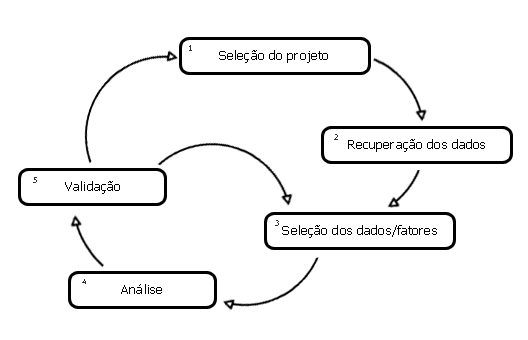
\includegraphics[width= .9\textwidth]{figuras/metodo_pesquisa}
    \caption{Método de pesquisa.}
    \label{fig:metodo}
 \end{figure}

A primeira etapa consiste da escolha do projeto de software livre. Posteriormente, no Passo 2, são recuperados os dados do projeto escolhido para que, na próxima etapa, seja iniciada de fato a mineração dos dados do repositório de software para fins de recomendação de especialistas.  No Passo 3 realiza-se a seleção dos dados e a identificação dos fatores a serem considerados para a recomendação de especialistas. Por exemplo, devem ser considerados fatores que classificam um desenvolvedor como veterano ou novato e as características dos artefatos recolhidos durante o Passo 2.

Cada desenvolvedor é analisado de forma individual com propósito de encontrar padrões e interesses. Esta análise compreende o Passo 4. Durante esta análise de padrões escolhe-se o algoritmo de recomendação de especialistas. Por último, no Passo 5, os resultados obtidos através desta recomendação devem ser validados, comparando-se com os casos reais de interação dos desenvolvedores, verificando-se a eficácia da recomendação de especialistas resultante.

Após a validação, existem duas possibilidades. A primeira é, no caso de resultados insatisfatórios, retornar ao Passo 3 para que seja feita outros testes em busca de novos resultados no mesmo projeto, refinando-se o algoritmo de recomendação. A segunda opção é voltar ao Passo 1, iniciando-se uma nova iteração para análise de outro projeto de software livre, verificando-se o modelo proposto também é valido para o novo projeto ou se ele precisa ser ajustado com novos parâmetros ou características ou ainda se modelos distintos devem ser extraídos para cada projeto.
 
\section{Seleção dos projetos}
\label{secao:metodo:selecao}

Diante da inviabilidade de analisar a grande massa de projetos OSS existentes, deve-se escolher projetos que tenham atributos suficientes para a recomendação de especialistas. Por exemplo, deve-se priorizar projetos com desenvolvedores especialistas, artefatos de qualidade e uma comunidade atrativa para novatos (por exemplo, projetos populares).

Estima-se que existiam mais de 500 mil projetos ativos de código aberto em julho de 2013 em todo o mundo. O número total de projetos é muito maior, mas não são todos que se encontram ativos~\cite{daffara}. Para identificar candidatos para análise, recomendamos o banco de dados do índice de projeto de código aberto Ohloh.net, um site que oferece um conjunto de serviços Web e plataforma de comunidade on-line que visa mapear o cenário de desenvolvimento de software de código aberto.

Segundo Kolassa et al. (2013)~\nocite{Kolassa-etal:2013}, deve-se levar em consideração um projeto ativo em um determinado ponto do tempo: quando o número de \textit{commits} (alterações feitas no código fonte da aplicação) nos últimos 12 meses é de pelo menos 60\% do número de \textit{commits} nos 12 meses antes disso; com uma história já traçada; objetivos claros; uma comunidade já bem estruturada e estabelecida; e versões já publicadas. Por exemplo: seria desejável um projeto com uma comunidade de no mínimo 50 desenvolvedores, com uma análise de testes estatísticos, uma ampla opção de comunicação, estabelecidos fóruns, listas de discussões e ferramentas de controle de versão para auxilio deste software.

\section{Seleção dos dados a serem extraídos}

Baseado na revisão realizada no \cref{cap:teoria}, observamos que os dados são geralmente recuperados dos comentários provenientes do gerenciador de tarefas do projeto, lista de discussões dos desenvolvedores e repositórios de código-fonte.

Segundo \citeonline{Robbes-etal:2013} estes repositórios e gerenciadores contém vários pontos de dados relevantes para métricas de especialistas. Por exemplo, o tempo que um desenvolvedor levou para realizar uma tarefa de desenvolvimento e edições, ou seja, a sequência de alterações de código que foram necessárias para executar a tarefa referida e as seleções ou os elementos de código que foram consultados durante a execução da tarefa.

A \cref{fig:classes} mostra o modelo conceitual dos artefatos relacionados com a MSR. Os desenvolvedores estão relacionados ao projeto de software por meio de suas listas de e-mail, repositório de código e gerenciadores de tarefas associado. Por meio do gerenciador de tarefas e listas de e-mail os desenvolvedores podem se comunicar com outros desenvolvedores do projeto. Correções e \textit{patch} (conjunto de alterações em arquivos de código fonte) também podem ser vinculadas com o desenvolvedor por meio do e-mail e comentários proveniente do gerenciador. 

\begin{figure}[hbt]
    \centering
    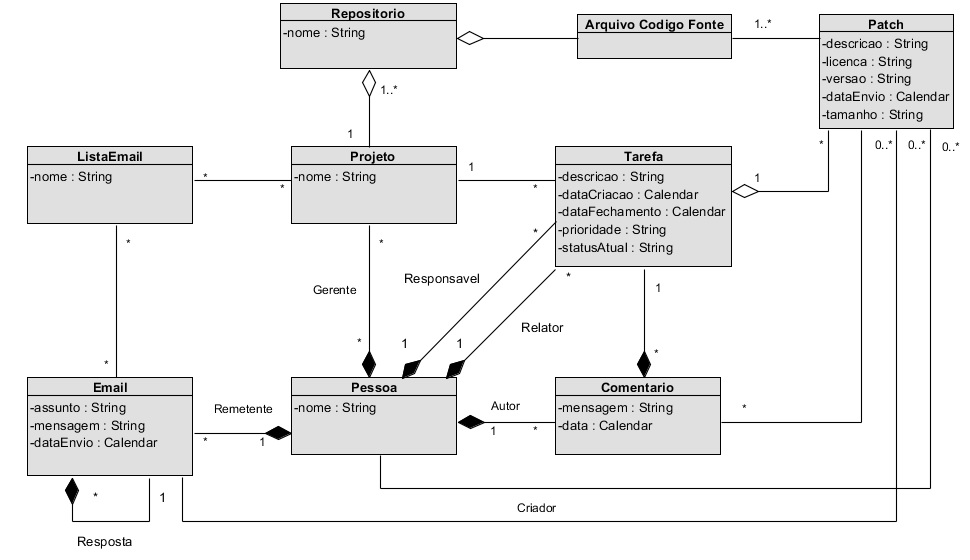
\includegraphics[width= .9\textwidth]{figuras/classes}
    \caption{Modelo conceitual dos dados a serem utilizados na MSR neste trabalho.}
    \label{fig:classes}
\end{figure}

Para a coleta dos dados do gerenciador de tarefas, recomenda-se a utilização de ferramentas de extração, tais como Bicho (\url{http://github.com/MetricsGrimoire/Bicho}), na qual realiza as chamadas ao Bugzilla e obtém as informações das tarefas e também as informações detalhadas dos comentários atrelados a elas.

Para realizar a extração do conteúdo de e-mails, primeiramente devem ser obtidos os arquivos que contém os e-mails de cada mês do período de análise. Estes arquivos incluem cabeçalho e mensagem. As informações das mensagens contidas nos cabeçalhos devem ser analisadas para adquirir informações do conteúdo da mensagem, anexos contendo \textit{patches}, assunto, ID da mensagem, remetente e identificador da cadeia de mensagens (\textit{In-reply-to}), que identifica a árvore de discussão (\textit{thread}) a qual a mensagem pertence. Essas árvores devem ser reconstruídas verificando o campo \textit{in-reply-to} do cabeçalho bem como o assunto do e-mail (examinando os prefixos \textit{``Re:", "Fwd:"}) e o campo "\textit{references}"  do cabeçalho, para diminuir as chances de perda de mensagens relativas a uma discussão.  Os \textit{patches} devem ser obtidos através dos anexos presentes nos e-mails e nas mensagens do gerenciador. Estes estão relacionados a um ou mais arquivos presentes no repositório de desenvolvimento de software. Com essas informações é possível identificar os responsáveis pelas correções e os associados com o envio. Para a análise devem ser desconsideradas as mensagens enviadas automaticamente na criação da tarefa, comentário ou mudança de estado das ferramentas de controle. Por fim, recomenda-se o armazenamento de e-mails em um banco de dados relacional.

Finalmente, as alterações de arquivos de código-fonte estão relacionadas aos arquivos armazenados no sistemas de controle de versão. Dessa forma, é possível conhecer as pessoas responsáveis por cada trecho de código existente no programa, dado esse útil para realizar a recomendação com base nos demais dados coletados.


\section{Seleção de dados e fatores}

A partir dos dados extraídos dos repositórios, devem ser selecionados aqueles que permitem identificar o tipo dos desenvolvedores -- novatos e veteranos/experientes -- e as características dos artefatos que permitem estabelecer o grau de experiência de cada desenvolvedor. A escolha desses fatores está relacionada aos algoritmos utilizados. Por exemplo, poderíamos utilizar o tempo médio entre realização de alterações no código fonte~\cite{Robbes-etal:2013}.

\section{Análise dos dados}

A análise dos dados capturados e armazenados devem passar por um processo de seleção descritiva. Esse processo consiste em examinar os dados com o objetivo de encontrar características e padrões relevantes sem que necessariamente exista uma ideia ou hipótese clara.

Os dados devem passar por um processo de filtragem, no geral descartando-se possíveis mensagens indesejadas contidas entre os dados coletados. O processo de análise inicialmente é otimizado por comandos SQL para realizar consultas no banco de dados, usando palavras-chave como filtros para que se possa reduzir a quantidade de tuplas nos resultados obtidos. Com uma parte das mensagens indesejadas já identificadas, o processo deve se repetir de forma manual, analisando atentamente os dados restantes. 

No momento seguinte deve-se identificar os desenvolvedores contidos tanto nas listas de discussões quanto nas ferramentas de gerenciamento de tarefas. Esses nomes necessitaram de ser agrupados de forma independente. A seguir, deve-se identificar a intersecção entre estes contidos nas listas e nas informações das ferramentas de controle, como demostrado na \cref{fig:int}. Os desenvolvedores contidos nesta intersecção, em parte por experiência adquirida e em parte por suas próprias observações, podem ser considerados  desenvolvedores experientes sobre os termos discutidos, por estarem envolvidos nas discussões decorrentes tanto no gerenciador de tarefas quanto nas listas de discussões.

\begin{figure}[!htb]
    \centering
    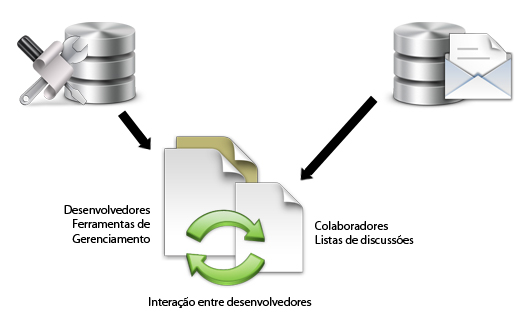
\includegraphics[width= .8\textwidth]{figuras/interacao}
    \caption{Agrupamento de desenvolvedores.}
    \label{fig:int}
\end{figure}

Passando para uma análise mais profunda, neste momento é necessária a utilização de algoritmos de identificações de padrões e interesses dos desenvolvedores selecionados. Para isso é preciso identificar as características relevantes dos novatos, desenvolvedores experientes e dos artefatos de software extraídos, de modo a definir o algoritmo de recomendação. Por exemplo, o algoritmo deve ser capaz de analisar palavras-chaves e arquivos de forma a agrupar uma série de informações sobre o desenvolvedor.  A frequência que estas palavras aparecem ao decorrer da análise demostrará o assunto mais debatido e trabalhado. Estas informações podem ser associadas a cada desenvolvedor agindo como uma espécie de perfil. 

A partir da lista de desenvolvedores, deve ser realizado a análise e a recomendação. Quando o novato começar a interagir com o projeto de software livre espera-se que mensagens sejam disparadas. Essas mensagens devem ser identificadas e então analisadas com base nas características pertinentes ao algoritmo. Caso seja possível realizar a identificação do componente do qual se trata a questão, o algoritmo de recomendação deve utiliza-la como base para relacionar o assunto. Caso não seja possível, então o algoritmo escolherá com base nas informações os desenvolvedores especialistas que mais tem relações com novatos em um ponto inicial do projeto. Esta recomendação deve ser considerada padrão caso não se encontre padrões na forma como o novato se expressou para começar a sua interação.


\section{Validação}

No geral, os trabalhos tendem a identificar especialistas com altos índices de alterações no código fonte (\textit{commits}), linhas de código e suas respostas. No entanto, não se leva em conta quanto tempo ele não tem mais interagido com estes artefatos. Para realizar esta análise é necessário um controle para que possa determinar a prioridade das indicações. O fator temporal considera técnicas indicadoras de decaimento para medir as interações de cada colaborador. Além disso, outro diferencial é a recomendação sendo direcionada para novatos que estão começando suas interações no projeto. Dessa forma, devemos verificar o quanto a abordagem de recomendação temporal será precisa nesses casos.  

Para essa análise deve ser realizada a coleta dos dados do projeto desde sua criação até a seis meses antes de sua data atual. Desenvolvedores que devem ser presentes até esta data devem ser considerados como experientes. Então uma nova análise com alvo nos últimos seis meses  identificará os novatos do projeto.
 
A recomendação de especialistas deve analisar cada mensagem ou tarefa dos novatos identificados para descobrir artefatos ou termos que permitam uma recomendação e então apresentar uma lista de desenvolvedores candidatos para responder este novato com uma prioridade de acordo com sua posição na lista, no qual o primeiro seria o mais indicado. 

Os modelos obtidos através do algoritmo devem ser comparados com exemplos reais de indicação do projeto escolhido, observando-se manualmente o especialista real com a indicação do algoritmo. 




\chapter{Resultados}
\label{cap:resultados}


\vspace{-1.5cm}
Nesta seção é relatada a execução do método proposto apresentando um mecanismo para recomendação de especialistas para novatos. Foram analisados dados provenientes de listas de discussões, interações em código fonte e gerenciadores de tarefas do projeto LibreOffice. Para realizar está análise foi desenvolvida uma ferramenta identificar padrões nestes meios de interações de desenvolvedores e sugerir especialistas para novatos.

A partir dos dados do projeto selecionado, deve-se possibilitar a ferramenta identificar os usuários presentes nos vários módulos de agrupamento de dados do projeto e transformar estes em uma estrutura relacional onde então é possível aplicar cálculos de experiência para seus contribuidores. A ferramenta consiste em três grandes processos: importação, processamento e apresentação de resultados.

A \cref{fig:process} apresenta os passos para a execução do algoritmo. A primeira etapa consiste em preparar os dados para o processamento. Existem duas grandes massas de dados: uma resultante dos relatos de erros obtidos através da ferramenta Bicho e outra proveniente da ferramenta de controle de versão Git. Os relatos de erros são recuperados do Bugzilla e armazenados em um banco de dados relacional definido pela ferramenta Bicho.

\begin{figure}[hb]
    \centering
    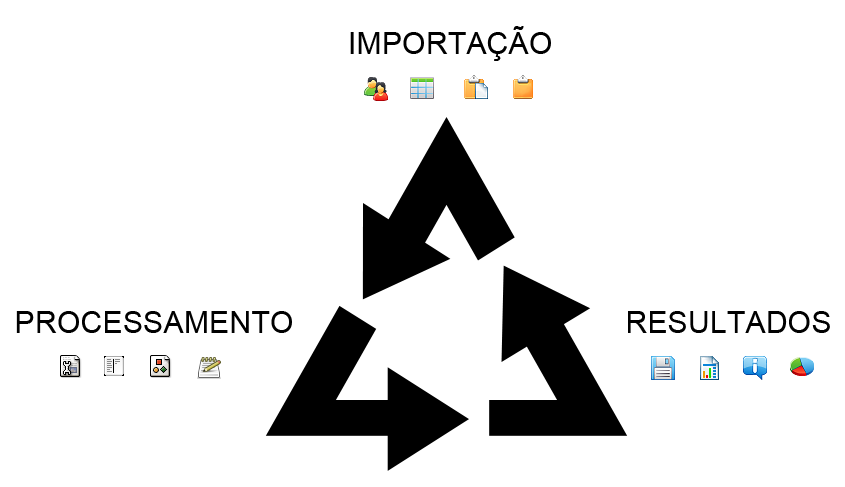
\includegraphics[width= .7\textwidth]{figuras/import}
    \caption{Estrutura de execução da ferramenta de recomendação.}
    \label{fig:process}
\end{figure}

Nas próximas seções, são descritos os resultados da aplicação do método definido no \cref{cap:metodo} e os componentes da ferramenta associados à geração de tais resultados.


\section{Seleção dos Projetos}

Para este trabalho, utilizou-se o software LibreOffice como objeto de estudo. O LibreOffice, uma ferramenta livre multiplataforma para escritório, surgiu como uma ramificação do projeto original OpenOffice.org, que, por sua vez, é oriundo do StarOffice 5.1. O código fonte da ferramenta foi liberado para que fosse possível a participação de contribuintes para desenvolvê-lo, dando início ao projeto de desenvolvimento de um software de código aberto em 13 de outubro de 2000, o OpenOffice.org. O LibreOffice surgiu a partir da versão 3.3, trazendo todas as características presentes no OpenOffice.org 3.3, além de outras tantas exclusivas do projeto LibreOffice. Sendo um projeto de código aberto seus dados estão disponíveis para a comunidade, as informações referentes a  relatos de erros (Bugzilla) estão disponíveis em \url{www.libreoffice.org/bugzilla} e o repositório Git esta disponível em \url{git://anongit.freedesktop.org/libreoffice/core}.

\section{Recuperação dos dados}

Neste projeto, foram utilizadas ferramentas de código aberto para realizar operações de 
recuperação dos dados em relatos de erros (\textit{issues}) e registros de alteração (\textit{commits}). As listas de relatos de erros foram  obtidas do repositório Bugzilla (\url{http://bugzilla.org}). Para essa extração foi utilizada uma ferramenta livre, desenvolvida em Python, denominada Bicho (\url{http://github.com/MetricsGrimoire/Bicho}). A ferramenta Bicho necessita de: (1) uma pré-configuração, na qual são necessários um registro no Bugzilla do projeto, pois a ferramenta necessita de autenticação para realizar a extração das informações; e (2) uma base de dados para receber toda a informação recuperada. Em relação às alterações no código fonte e os registros destas, foi utilizado o sistema de controle de versão Git (\url{http://git-scm.com}), tal como aqueles disponibilizados em agregadores de projetos de software livre como o GitHub (\url{http://github.com}). 

Nos dados obtidos se apresentam: usuários, relatos, comentários e descrição. Com o auxílio da ferramenta construída, a importação consistiu em inicialmente recuperar os usuários dos dois grandes agrupamentos de dados. As informações armazenadas no banco de dados MySQL criada pela ferramenta Bicho foram importadas realizando consultas na base e reestruturando as informações como apresenta na \cref{fig:bd-bicho}. A importação consistiu em utilizar o Hibernate, um framework para o mapeamento de objetos para modelos relacionais construído em Java, para que os dados agora transformados em informações fossem salvos. 

\begin{figure}[hbt]
    \centering
    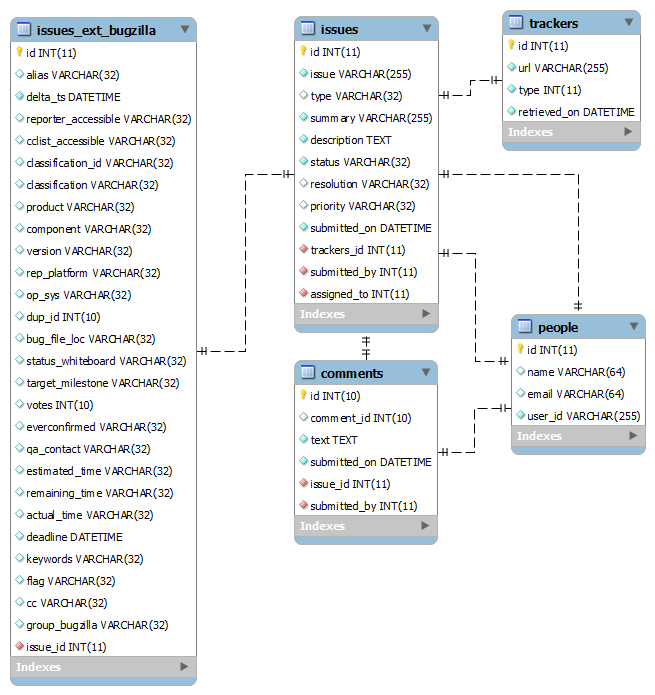
\includegraphics[width=.58\textwidth]{figuras/bicho}
    \caption{Principais entidades definidas na base de dados criada pela ferramenta Bicho.}
    \label{fig:bd-bicho}
 \end{figure}

Após a importação dos usuários providos dos relatos de erros, foi necessário importar os usuários presentes no código fonte. O processo foi similar, mas utilizando uma ferramenta denominada de Jgit, um plugin desenvolvido pelo Eclipse para manipulação de repositórios Git. Este módulo do software, ilustrado na \cref{fig:impu}, é responsável por fazer a leitura no repositório do projeto armazenado localmente e importar os usuários, mesclando com os já presentes provenientes dos relatos de erros.

\begin{figure}[hbt]
    \centering
    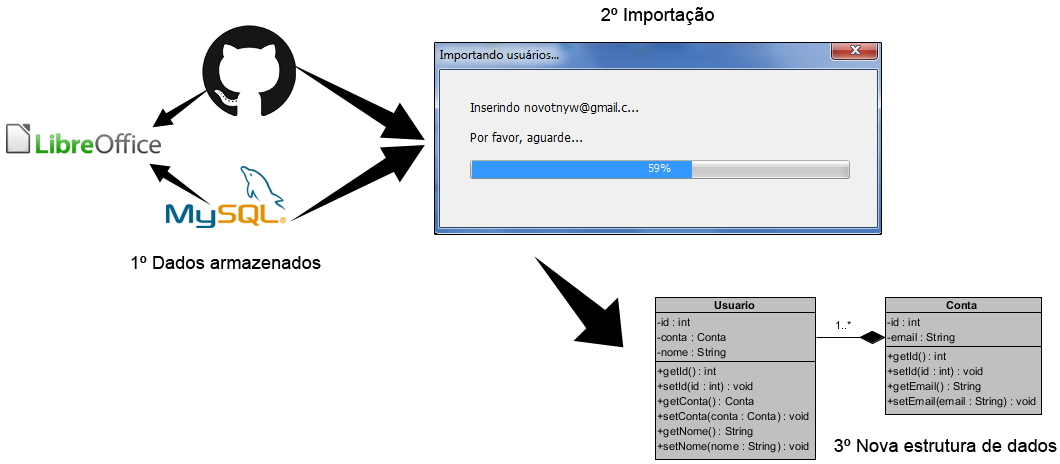
\includegraphics[width=.95\textwidth]{figuras/impe}
    \caption{Processo de importação de usuários provenientes do projeto.}
    \label{fig:impu}
\end{figure}

O processo foi realizado de forma similar nos outros componentes presentes na estrutura relacional, resultando em importar os dados provenientes dos relatos de erros, comentários e código fonte. A estrutura resultante será onde a algoritmo realizará leituras para a recomendação. A \cref{fig:diagE} mostra o resultado final desta operação. 

\begin{figure}[hbt]
    \centering
    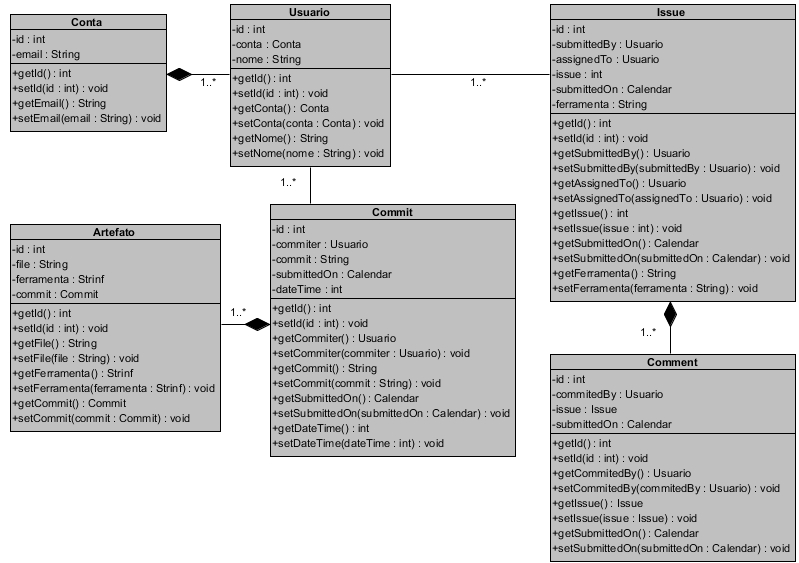
\includegraphics[width=.95\textwidth]{figuras/diagramaF}
    \caption{Estrutura de dados relacional.}
    \label{fig:diagE}
\end{figure}

O processo de importação foi necessário para que o algoritmo possuísse um desempenho melhor. Após testes de execução com os dados gerados sem uma preparação, foi notável o seu fraco desempenho devido ao grande número de consultas necessárias para realizar tarefas simples. Após o rearranjo destes dados foi possível acessar as informações de forma mais rápida, diminuindo seu tempo de execução. Ainda quanto à importação, é necessário estabelecer a relação entre \texttt{issues} e \texttt{commits}. Para a identificação dos componentes, tal como apresentados nas \texttt{issues} e as alterações nos arquivos de código fonte, através dos \texttt{commits} realizados pelos desenvolvedores, foi necessário identificar um padrão entre diretórios em que tais arquivos estavam presentes e os componentes das \texttt{issue} do projeto. No caso da ferramenta, este mapeamento está implementado no código, sendo específico para a projeto sob análise.

O projeto analisado possui uma rica quantidade de dados. Com o auxílio da ferramenta foram recuperados dados relacionados ao código fonte até 31/12/2012 constituindo uma base de dados de 154.381 registro de interações no código fonte do projeto. Foram coletados relatos de erros até 31/12/2012, totalizando 10.187 relatos de erros presentes na ferramenta de controle Bugzilla e 57204 comentários a estes relatos.  Os desenvolvedores presentes no projeto foram mesclados entre código fonte e relatos de erros. No total foram identificados 6.685 registros de contas de usuário no projeto desde seu inicio até a data de análise dos dados recuperados.

As datas iniciais variam entre os registros de erros e de alterações no código fonte: os relatos de erros possuem seu primeiro registro em 03/08/2010 enquanto o código fonte possui seu primeiro \textit{commit} em 02/01/2008. Alguns registros relacionados a \textit{commit} foram descartados devido ao início do projeto e do grande número de \textit{commit} para estabelecer o desenvolvimento proveniente do código oriundo do OpenOffice. Analisando as datas é notável que inicialmente poderiam existir dois universos. O primeiro seria uma baixa quantidade de colaboradores no projeto e uma comunicação fácil, não necessitando no momento de uma ferramenta externa para controle de problemas relacionado ao projeto, pois entre a data do primeiro relato para o primeiro \textit{commit} foram 2 anos de diferença. Outra hipótese poderia ser o funcionamento do projeto estar paralisado e então tomado o seu desenvolvimento a partir de 2010, onde desenvolvedores pertencentes ao OpenOffice começaram suas contribuições no projeto novo, migrando de uma ferramenta para outra.

\section{Seleção dos dados e fatores}

A terceira etapa consistiu em realizar o processamento das informações agrupadas na base criada pela ferramenta e relacionar os dados e fatores para a recomendação. Para a recomendação, o utilizador da ferramenta possui alguns filtros para refinar a sua recomendação, sendo possível escolher datas específicas. A recomendação é baseada nos artefatos do projeto, às quais o utilizador tem a opção de escolher as ferramentas disponíveis deste projeto e realizar a recomendação.

O processo de recomendação consiste em recuperar todos os usuários presentes na base de dados e realizar a contagem das interações do usuário no projeto e aplicando a fórmula específica para aquela ocasião. No caso, a formula escolhida na tela de seleção. Nesta etapa foi identificados problemas pois a ferramenta precisou ser modificada para utilizar classes específicas para cálculos matemáticos de grande precisão, pois soluções disponíveis na linguagem padrão não obteve sucesso em realizar tais operações. Apos aplicar a formula para todos os usuários o sistema apresenta uma lista de possíveis especialistas para o artefato em questão, ordenada de acordo com a sua experiência no artefato escolhido. A \cref{fig:ferra} apresenta a ferramenta, que contém no menu superior os comando para iniciar a recomendação do especialista e o processo de importação e pré-processamento para a recomendação. Estes últimos consistem na preparação da base de dados que tem o propósito de importar os dados provenientes do Git e dos relatos de erros armazenados no banco de dados do Bicho. A ferramenta possibilita também realizar uma busca na base completa identificando o especialista de maior participação naquele componente. Por fim temos os componentes presentes no projeto, que foram mapeados dos relatos de erros para o código fonte onde cada diretório do seu fonte representa parte de um componente presente nos relatos, podendo possuir cardinalidades 1 para N. A ferramenta se encontra disponível no GitHub (\url{https://github.com/ehrickwilliam/Minerador}).

\begin{figure}[bt]
    \centering
    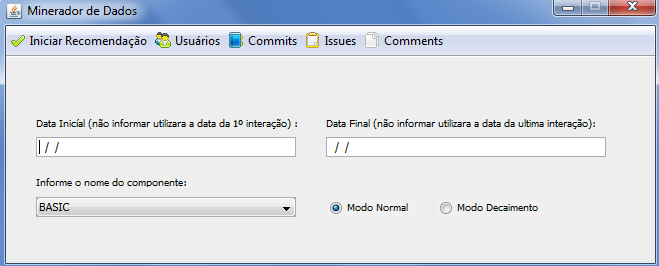
\includegraphics[width=.8\textwidth]{figuras/ferramenta}
    \caption{Ferramenta de recomendação.}
    \label{fig:ferra}
\end{figure}


Para a identificação dos componentes presentes no código fonte, através dos commits realizados pelos desenvolvedores foi necessário identificar um padrão entre diretórios e componentes do projeto. Para isto foi utilizada a documentação online disponível do LibreOffice (\url{http://docs.libreoffice.org/}) para realizar um mapeamento nos diretórios do código fonte manipulados pelo commit e identificar qual componente aquele commit está relacionado. Apos analise definiu-se o mapeamento apresentado na \cref{tab:mapeamento}.

\begin{table}[htb]
    \centering
    \scriptsize
    \caption{Mapeamento entre componentes e diretórios com arquivos de código fonte.}
    \label{tab:mapeamento}
    \subfloat[][]{
        \begin{tabular}{|l|l|}
            \hline
                \textbf{Componente}    & \textbf{Diretórios}\\\hline
                    BASIC  & /core/basic \\\hline
                           & /core/basctl \\\hline
                    Chart  & /core/chart2 \\\hline
%                    contrib  &  \\\hline
                    Database  & /core/connectivity \\\hline
                           & /core/configmgr \\\hline
                           & /core/dbaccess \\\hline
%                    Documentation  &  \\\hline
                    Drawing  & /core/drawinglayer \\\hline
                           & /core/sd \\\hline
                    Extensions  & /core/odk \\\hline
                           & /core/extensions \\\hline
                    Filters e Storage  & /core/sot \\\hline
                           & /core/xmlsecurity \\\hline
                           & /core/filter \\\hline
                           & /core/xmloff \\\hline
                           & /core/binfilter \\\hline
                           & /core/lotuswordpro \\\hline
                    Formula Editor  & /core/starmath \\\hline
                    Framework  & /core/framework \\\hline
                           & /core/wizards \\\hline
                           & /core/ucbhelper \\\hline
                           & /core/io \\\hline
                    Graphics stack  & /core/svx \\\hline
                    Installation  & /core/readlicense\_oo \\\hline
                           & /core/scp2 \\\hline
                           & /core/instsetoo\_native \\\hline
                \end{tabular}
        } 
        \qquad
        \subfloat[][]{          
            \begin{tabular}{|l|l|}
                \hline
                \textbf{Componente}    & \textbf{Diretórios}\\\hline
                    Libreoffice  & /core/desktop \\\hline
                    Linguistic  & /core/Linguistic \\\hline
                    Localization  & /core/l10ntools \\\hline
                    Presentation  & /core/slideshow \\\hline
                           & /core/sdext \\\hline
%                    Printing and PDF export  & \\\hline
                    sdk  & /core/test \\\hline
                           & /core/testautomation \\\hline
                           & /core/offapi \\\hline
                           & /core/qadevOOo \\\hline
                           & /core/formula \\\hline
                    Spreadsheet  & /core/sc \\\hline
                    UI  & /core/uui \\\hline
                            & /core/dmake \\\hline
                            & /core/svtools \\\hline
%                            & /core/ooo\_custom\_images \\\hline
                            & /core/cui \\\hline
                            & /core/default\_images \\\hline
                            & /core/forms \\\hline
                            & /core/icon-themes \\\hline
                            & /core/accessibility \\\hline
                            & /core/extras \\\hline
                    Writer  & /core/sw \\\hline
                        & /core/swext \\\hline
                        & /core/writerfilter \\\hline
                        & /core/writerperfect \\\hline
%                    WWW  &  \\\hline
        \end{tabular}
    }
\end{table}

Tendo o principal objetivo de propor melhores resultados para novatos no sistema de recomendação, foi necessário identificá-los entre usuários do projeto. Este processo constituiu em integrar as informações provenientes das \textit{issues} e listas de e-mail. Nesta última se concentram a maioria das interações iniciais dos novatos. Para este procedimento assumimos as seguintes heurísticas:

\begin{itemize}
    \item Usuários experientes:, desenvolvedores que possuem interações com alguma ferramenta do projeto nas datas iniciais de analise até Junho de 2012.
    \item Usuários novatos: possuem interações apenas entre Julho de 2012 até Dezembro de 2012.
\end{itemize}

A identificação dos novatos presentes nas interações citadas seguiu o seguinte procedimento: oriundos das listas e de e-mails e \textit{issues}, meios principais de inicio de colaboração em um projeto de código aberto por novatos. Neste procedimento foi ignorado a interação de novatos a partir de \textit{commits}, dado que, normalmente, limita-se a desenvolvedores experientes o acesso para inclusão de alterações de código fonte no repositório, concentrando-se as interações de novatos principalmente por esses dois meios relatados na análise. Foram selecionados 2 grupos, o primeiro constituído por usuários com interações até Junho de 2012 e o segundo grupo com interações de Julho até Dezembro de 2012. Com estes grupos então foi criado uma intersecção gerando o terceiro grupo contendo apenas desenvolvedores que não pertencem ao primeiro grupo, dando origem aos novatos do projeto. Foi necessária uma ferramenta para realizar a importação dos e-mails disponíveis online pelo LibreOffice, entre as ferramentas existentes para realizar este procedimento, optamos pela ferramenta Presley (\url{https://github.com/magsilva/presley}) desenvolvida em Java \cite{Trindade-etal:2009}. Está realizou a importação dos arquivos de e-mails (.mbox) em um modelo relacional. Neste modelo utilizamos 3 (três) entidades: desenvolvedor, problema e solução. Desenvolvedor representa quem interagiu com esta lista. Problema é considerado o primeiro e-mail e solução as respostas que este e-mail possuiu. 


\section{Análise dos dados}

A partir dos usuários identificados seguimos três abordagens. A primeira constituiu em uma lista de desenvolvedores utilizando como parâmetro de ordenação mais \textit{issues} e mais e-mails. Desta forma obtemos uma lista constituída por 5 (cinco) novatos. Da segunda abordagem recuperamos os 5 (cinco) novatos com mais e-mails e mais \textit{issues}. A última constituiu na intersecção destas duas lista, gerando 5 (cinco) novatos supostamente bem sucedidos, como apresentado a \cref{tab:novatossucedidos}.

\begin{table}[hbt]
    \centering
    \scriptsize
    \caption{Relação de novatos mais promissores.}
    \label{tab:novatossucedidos}
    \begin{tabular}{|l|c|c|l|}
        \hline
                \textbf{Novatos} & \textbf{Issues} & \textbf{E-mails}  & \textbf{Componentes}\\\hline
                   nickshanks@nickshanks.com  & 2 & 3 & UI, Libreoffice, Installation\\\hline
                   lbalbalba@gmail.com        & 0 & 106 & SDK\\\hline
                   ruderphilipp@gmail.com     & 0 & 26 & Spreadsheet\\\hline
                   ttk448@gmail.com           & 0 & 22 & Spreadsheet\\\hline
                   uray.janos@gmail.com       & 0 & 13 & Framework\\\hline
    \end{tabular}
\end{table}

Com a relação dos novatos bem sucedidos, verificamos os desenvolvedores responsáveis pelas respostas nos meios no qual eles interagiram. Neste caso foi computada a quantidade de vezes que o desenvolvedor veterano interagiu no tópico do novato e ordenado pelo maior numero de interações. Os desenvolvedores presentes nas \cref{tab:novatosissue} e \cref{tab:novatosrec} são considerados a recomendação real e os candidatos para a validação da ferramenta automatizada para recomendação de especialistas para novatos.

\begin{table}[hbt]
    \centering
    \scriptsize
    \caption{Relação de recomendações para issues.}
    \label{tab:novatosissue}
    \begin{tabular}{|l|c|c|c|}
        \hline
                \textbf{Novatos}
                & \textbf{Pos.}
                & \textbf{Desenvolvedores}
                & \textbf{Total}\\\hline
                    nickshanks@nickshanks.com   & 1º & sbergman@redhat.com & 4\\\hline
                                                & 1º & bfo.bugmail@spamgourmet.com & 4\\\hline
                                                & 2º & tlillqvist@suse.com & 3\\\hline
                                                & 3º & scren2004@yahoo.de & 1\\\hline
                                                & 3º & bugs@eikota.de & 1\\\hline
    \end{tabular}
\end{table}


\begin{table}[hbt]
    \centering
    \scriptsize
    \caption{Relação de recomendações para e-mails.}
    \label{tab:novatosrec}
    \begin{tabular}{|l|c|c|c|}
        \hline
                \textbf{Novatos}
                & \textbf{Pos.}
                & \textbf{Desenvolvedores}
                & \textbf{Total}\\\hline
                    nickshanks@nickshanks.com   & 1º & caolanm@redhat.com & 2\\\hline
                                                & 1º & tml@iki.fi & 2\\\hline
                                                & 1º & heinzlesspam@gmail.com & 2\\\hline
                    lbalbalba@gmail.com         & 1º & sbergman@redhat.com & 14\\\hline
                                                & 2º & vmiklos@collabora.co.uk  & 10 \\\hline
                                                & 3º & dtardon@redhat.com  & 6 \\\hline
                                                & 4º & matus.kukan@collabora.com  & 4 \\\hline
                                                & 4º & noelgrandin@gmail.com  & 4 \\\hline
                                                & 5º & caolanm@redhat.com  & 3 \\\hline
                                                & 5º & olivier.hallot.tdf@gmail.com  & 3 \\\hline
                                                & 5º & bjoern.michaelsen@canonical.com  & 3 \\\hline
                                                & 5º & mst@openoffice.org  & 3 \\\hline
                    ruderphilipp@gmail.co       & 1º & nopower@novell.com & 7\\\hline
                                                & 2º & johann.messner@jku.at & 5\\\hline
                                                & 2º & erack@redhat.com & 5\\\hline
                                                & 3º & jmadero.dev@gmail.com & 4\\\hline
                                                & 4º & lohmaier+ooofuture@googlemail.com & 3\\\hline
                                                & 5º & tenger@iseries-guru.com & 2\\\hline
                                                & 6º & caolanm@redhat.com & 1\\\hline
                                                & 6º & jnabet2412@free.fr & 1\\\hline
                                                & 6º & rb.henschel@t-online.de & 1\\\hline
                                                & 6º & noelgrandin@gmail.com & 1\\\hline
                    ttk448@gmail.com            & 1º & erack@redhat.com & 7\\\hline
                                                & 1º & kohei.yoshida@collabora.com & 7\\\hline
                                                & 1º & markus.mohrhard@googlemail.com & 7\\\hline
                                                & 2º & mst@openoffice.org & 3\\\hline
                                                & 3º & andrew@pitonyak.org & 1\\\hline
                                                & 3º & michael.meeks@suse.com & 1\\\hline
                                                & 3º & sbergman@redhat.com & 1 \\\hline
                    uray.janos@gmail.com        & 1º & tml@iki.fi & 4\\\hline
                                                & 2º & noel.power@gmail.com & 3\\\hline
                                                & 3º & vmiklos@collabora.co.uk & 2\\\hline
                                                & 3º &caolanm@redhat.com & 2\\\hline
                                                & 3º &timar@fsf.hu & 2\\\hline
                                                & 4º &sbergman@redhat.com & 1\\\hline
                                                & 4º &mst@openoffice.org & 1\\\hline

    \end{tabular}
\end{table}




No processo de estruturação dos dados foi necessário implementar funções na ferramenta proposta para realizar a automação dos dados e mapear para um banco de dados relacional. Tal estrutura foi criada para execução dos algoritmos de mineração de repositório e para a implementação do sistema de recomendação. A \cref{fig:est} mostra a estrutura após o processamento dos dados, em que o usuário esta relacionado com sua conta e este pode possuir interações no projeto na forma de relatos de erros (\textit{issue}), comentários e registros de alteração (\textit{commits}).

\begin{figure}[!htb]
    \centering
    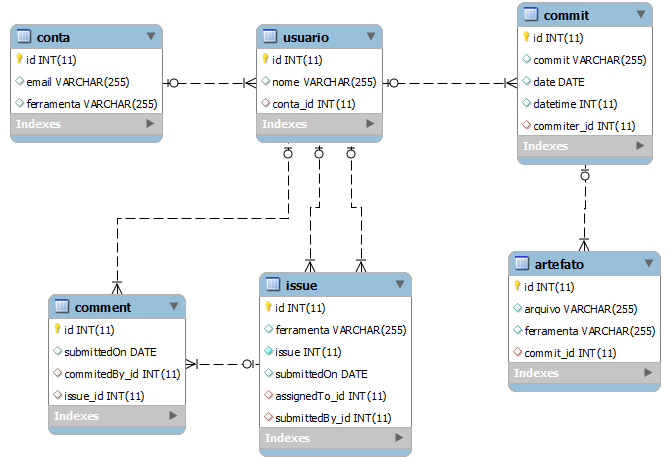
\includegraphics[width= .8\textwidth]{figuras/tabelas_banco}
    \caption{Estrutura relacional do banco de dados.}
    \label{fig:est}
\end{figure}


Os dados recuperados através da ferramenta Bicho possibilitaram a população das entidades \texttt{issue} e \texttt{comment}. A entidade \texttt{commit} foi obtida através dos dados recuperados da ferramenta Git e da clonagem do repositório do projeto. A entidade \texttt{artefatos} foi definida utilizando a entidade \texttt{commit} e recuperando os artefatos modificados na árvore de dados de cada \texttt{commit}, submetendo-os ao mapeamento composto por diretório do arquivo de código fonte alterado e o componente registrado em \texttt{issue} (atributo \texttt{ferramenta}). Tal mapeamento, por enquanto, é realizado manualmente.

Em relação aos algoritmos de recomendação, comparamos duas métricas para ilustrar nossa abordagem: a primeira avalia a experiência de um desenvolvedor dada uma ação em um artefato com a quantidade de alterações (\texttt{commits}) e relatos de erros em que ele colaborou. A segunda abordagem considera que  as alterações recentes possuem pesos maiores na hora de avaliar um desenvolvedor em determinado artefato. Ambas as abordagens foram adaptadas do trabalho de \citeonline{Robbes-etal:2013}.

A abordagem utilizada neste trabalho consiste em agregar uma nova estrutura de dados a estas métricas, utilizando a combinação de \textit{commits} e \textit{issues} como fonte de alimentação para a experiencia dos desenvolvedores. A utilização dos dados provenientes das \textit{issues} nos proporciona dados de desenvolvedores mais comunicativos do que apenas desenvolvedores restritos a realizar \textit{commits} no projeto, os quais são uma pequena parcela do todo. Desta forma espera-se que as recomendações que incluam estas duas estruturas se tornem melhores. 

Nesta primeira abordagem é acrescentado 1 (um) a cada alteração no código fonte, relatos e comentário realizado pelo desenvolvedor para cada artefato. Tal acréscimo é feito sempre que um autor realizar uma alteração até uma data informada como parâmetro ao sistema de recomendação. Após esta etapa, é realizado o cálculo de experiência do desenvolvedor em relação ao artefato. Este procedimento utiliza a soma de todos os desenvolvedores e o valor acumulado então dividindo pelo seu total acumulado.

A \cref{fig:exp1} representa o procedimento utilizado para calcular a experiência.  Nossos indicadores de especialização são definidos em um ponto no tempo e para um determinado desenvolvedor. No instante $t$, para obter a experiencia de desenvolvedor $d$ na entidade código fonte, relato de erro ou comentário $e$, faz-se o cálculo sobre a soma do experiencia de cada um dos colaboradores, produzindo um valor de experiencia entre 0 e 1. Em outras palavras, o método simplesmente realiza a soma de \texttt{commits} e \texttt{issues} que o desenvolvedor realiza no projeto até uma determinada data e a compara com o total destes realizados no projeto.


\begin{figure}[hbt]
$$
    Exp(d, e, t) = \frac{ExpNaive(d, e, t)}{\sum_{d' \in D} ExpNaive(d', e, t)}
$$

$$
    ExpNaive(d, e, t)  = \sum_{c' \in C} WN(c', d, e, t)
$$

$$
    Valid(c, d, e, t) = Author(c,d) \land Changes(c, e) \land Date(c) > t
$$

$$
    WN(c, d, e, t) = \left\{
        \begin{array}{l l}
            1  & , Valid(c, d, e, t) = true\\
            0  & , Valid(c, d, e, t) = false\\
        \end{array} \right.
$$
    \caption[Técnica de recomendação sem temporalidade.]{Técnica de recomendação sem temporalidade por \citeonline{Robbes-etal:2013}.}

    \label{fig:exp1}
\end{figure}

Estas informações nos possibilitam realizar uma classificação em que os 10 (dez) primeiros são considerados especialistas no artefato escolhido. Por exemplo, na \cref{fig:processNormal}  temos uma recomendação utilizando o componente \texttt{Basic} do LibreOffice, demostrando o nível de contribuição dos especialistas, neste caso o usuário \url{caolanm@redhat.com} é considerado o mais experiente no artefato.

\begin{figure}[!htb]
    \centering
    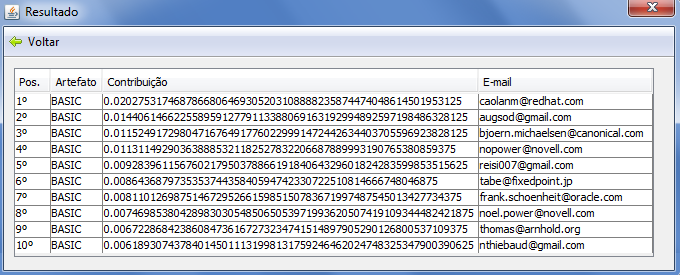
\includegraphics[width= .9\textwidth]{figuras/resultadoNormal}
    \caption{Resultado da recomendação segundo a primeira abordagem (modo normal).}
    \label{fig:processNormal}
\end{figure}

A segunda abordagem aplica técnicas de decaimento para as modificações mais recentes. Diferente da primeira abordagem esta técnica não realiza uma soma simples em que era possível obter apenas valores entre 0 e 1, mas utiliza uma análise temporal que incorpora a equação melhores pontos para modificações mais recentes. Esta técnica propicia um valor mais justo quanto a experiência de um desenvolvedor quanto a um artefato. 

Na \cref{fig:exp2} é apresentado o algoritmo da segunda abordagem. Esta técnica também conta o número de mudanças realizadas pelo desenvolvedor $d$ no artefato $e$ a partir do instante $t$, mas também se aplica o fator de decaimento: o peso da cada interação (\texttt{commit} ou \texttt{issue}) $c$ é 1, dividido pelo número de dias entre data da interação até a data atual. As alterações antigas têm um peso menor do que as mudanças recentes, mostrando a tendência das pessoas a esquecer de o que aprenderam ao longo do tempo.

\begin{figure}[hbt]
$$
    Exp(d, e, t) = \frac{ExpDecay(d, e, t)}{\sum_{d' \in D} ExpDecay(d', e, t)}
$$

$$
    ExpDecay(d, e, t)  = \sum_{c' \in C} WD(c', d, e, t)
$$

$$
    Valid(c, d, e, t) = Author(c,d) \land Changes(c, e) \land Date(c) > t
$$

$$
    WD(c, d, e, t) = \left\{
        \begin{array}{l l}
            \frac{1}{t-Date(c)}  & , Valid(c, d, e, t) = true\\
            0  & , Valid(c, d, e, t) = false\\
        \end{array} \right.
$$
    \caption[Técnica de recomendação com aspectos temporais.]{Técnica de recomendação com aspectos temporais por \citeonline{Robbes-etal:2013}.}
  
    \label{fig:exp2}
\end{figure}


Na \cref{fig:processExp}  temos a recomendação utilizando o mesmo componente \texttt{Basic} do LibreOffice, demostrando o nível de contribuição. Neste caso o usuário \url{caolanm@redhat.com} antes considerado o mais experiente no artefato acabou não sendo considerado um dos 10 (dez) melhores qualificados. Já o usuário \url{nopower@novell.com}, passou de 5º no modo anterior para o usuário com experiencia aplicando técnicas temporais.

\begin{figure}[!htb]
    \centering
    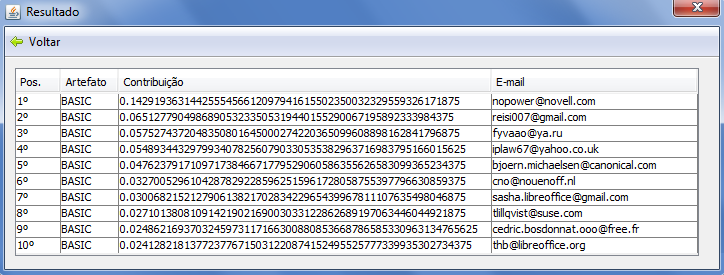
\includegraphics[width=\textwidth]{figuras/resultadoExp}
    \caption{Resultado da recomendação de acordo com a segunda abordagem (modo com decaimento).}
    \label{fig:processExp}
\end{figure}

\section{Validação}

O processo de validação constituiu em utilizar os componentes identificados nas \textit{issues} e nos e-mails. Diferente das \textit{issues}, em que os componentes estão presentes nas informações recuperadas, é necessário inferir os componentes tratados nos e-mails. Componentes relacionado aos e-mails foram identificados manualmente para os novatos selecionados, analizando-se as  mensagens trocadas para identificar qual o seu interesse no projeto e extrair o componente destas informações. Identificados os componentes, a ferramenta de recomendação foi executada, utilizando nossas duas abordagens de recomendação, obtendo-se os desenvolvedores especialistas presentes na \cref{tab:devrec} para os novatos selecionados.

\begin{table}[htb]
    \centering
    \scriptsize
    \caption{Relação de especialistas para novatos.}
    \label{tab:devrec}
    \begin{tabular}{|l|c|c|c|}
        \hline
                \textbf{Novatos}
                & \textbf{Pos.}
                & \textbf{Desenvolvedores (Temporal)}
                & \textbf{Desenvolvedores (Normal)}\\\hline
        nickshanks@nickshanks.com & 1º & caolanm@redhat.com & reisi007@gmail.com\\\hline
                                  & 2º & tlillqvist@suse.com & bjoern.michaelsen@canonical.com\\\hline
                                  & 3º & sebastian@sspaeth.de & caolanm@redhat.com\\\hline
                                  & 4º & bjoern.michaelsen@canonical.com & sbergman@redhat.com\\\hline
                                  & 5º & michael.meeks@collabora.com & michael.meeks@collabora.com\\\hline
                                  & 6º & libreoffice@kohei.us & tlillqvist@suse.com\\\hline
                                  & 7º & thb@libreoffice.org & sasha.libreoffice@gmail.com\\\hline
                                  & 8º & pmladek@suse.cz & bugs@eikota.de\\\hline
                                  & 9º & reisi007@gmail.com & pmladek@suse.cz\\\hline
                                  & 10º& nopower@novell.com & cno@nouenoff.nl\\\hline
        lbalbalba@gmail.com       & 1º & e1322577@rtrtr.com & frank.schoenheit@oracle.com\\\hline
                                  & 2º & iplaw67@yahoo.co.uk & jsk@openoffice.org\\\hline
                                  & 3º & eugene.kinyapin@gmail.com & bjoern.michaelsen@canonical.com\\\hline
                                  & 4º & mstahl@redhat.com & liuzhe@apache.org\\\hline
                                  & 5º & sbergman@redhat.com & mstahl@redhat.com\\\hline
                                  & 6º & mperkin5@csc.com & sbergman@redhat.com\\\hline
                                  & 7º & lionel@mamane.lu & noel@peralex.com\\\hline
                                  & 8º & jan.keirse@tvh.com & arist@apache.org\\\hline
                                  & 9º & r0polach@gmail.com & caolanm@redhat.com\\\hline
                                  & 10º& mprizsi-libreoffice@yahoo.com & Wolfram.Garten@oracle.com\\\hline
        ruderphilipp@gmail.co     & 1º & libreoffice@kohei.us & markus.mohrhard@googlemail.com\\\hline
                                  & 2º & markus.mohrhard@googlemail.com & libreoffice@kohei.us\\\hline
                                  & 3º & reisi007@gmail.com & kyoshida@novell.com\\\hline
                                  & 4º & bjoern.michaelsen@canonical.com & kohei.yoshida@suse.com\\\hline
                                  & 5º & sasha.libreoffice@gmail.com & reisi007@gmail.com\\\hline
                                  & 6º & cno@nouenoff.nl & kohei.yoshida@gmail.com\\\hline
                                  & 7º & nopower@novell.com & caolanm@redhat.com\\\hline
                                  & 8º & erack@redhat.com & erack@redhat.com\\\hline
                                  & 9º & bugs@eikota.de & bjoern.michaelsen@canonical.com\\\hline 
                                  & 10º & vitriol\_vitriol@katamail.com & sasha.libreoffice@gmail.com \\\hline 
        ttk448@gmail.com          & 1º & libreoffice@kohei.us & markus.mohrhard@googlemail.com\\\hline
                                  & 2º & markus.mohrhard@googlemail.com & libreoffice@kohei.us\\\hline
                                  & 3º & reisi007@gmail.com & kyoshida@novell.com \\\hline
                                  & 4º & bjoern.michaelsen@canonical.com & kohei.yoshida@suse.com \\\hline
                                  & 5º & sasha.libreoffice@gmail.com & reisi007@gmail.com \\\hline
                                  & 6º & cno@nouenoff.nl & kohei.yoshida@gmail.com \\\hline
                                  & 7º & nopower@novell.com & caolanm@redhat.com \\\hline
                                  & 8º & erack@redhat.com & erack@redhat.com\\\hline
                                  & 9º & bugs@eikota.de & bjoern.michaelsen@canonical.com \\\hline
                                  & 10º& vitriol\_vitriol@katamail.com & sasha.libreoffice@gmail.com \\\hline
        uray.janos@gmail.com      & 1º & cno@nouenoff.nl & anistenis@gmail.com \\\hline
                                  & 2º & sbergman@redhat.com & caolanm@redhat.com \\\hline
                                  & 3º & reisi007@gmail.com & bjoern.michaelsen@canonical.com \\\hline
                                  & 4º & michael.meeks@collabora.com & frank.schoenheit@oracle.com \\\hline
                                  & 5º & libreoffice@kohei.us & sbergman@redhat.com \\\hline
                                  & 6º & serval2412@yahoo.fr & noel@peralex.com \\\hline
                                  & 7º & bjoern.michaelsen@canonical.com & thomas@arnhold.org \\\hline
                                  & 8º & pmladek@suse.cz & sb@openoffice.org \\\hline
                                  & 9º & prlw1@cam.ac.uk & cd@openoffice.org \\\hline
                                  & 10º & drichard@largo.com & nthiebaud@gmail.com \\\hline


    \end{tabular}
\end{table}
\clearpage

A partir dos desenvolvedores que interagiram com os novatos e as recomendações pela ferramenta, foi construída a \cref{tab:novatovalidacao} que possui a intersecção para determinar os resultados da recomendação automática. Nos componentes analisados, ambas as abordagens obtiveram resultados presentes nas recomendações reais. Entretanto estes resultados possuem dois pontos de interpretação.

\begin{table}[hbt]
    \centering
    \scriptsize
    \caption{Intersecção de recomendações.}
    \label{tab:novatovalidacao}
    \begin{tabularx}{\textwidth}{|X|c|X|c|X|c|X|}
        \hline
                \textbf{Novatos}
                & \textbf{Pos.}
                & \textbf{Desenvolvedores (reais)}
                & \textbf{Pos.}
                & \textbf{Desenvolvedores (temporal)}
                & \textbf{Pos.}
                & \textbf{Desenvolvedores (normal)}\\\hline
                nickshanks@ nickshanks.com  & 1º & sbergman@redhat.com (issues)         & 1º &  caolanm@redhat.com   & 3º & caolanm@redhat.com\\\hline
                                           & 1º & bfo.bugmail @spamgourmet.com (issues) & 2º &  tlillqvist@suse.com  & 4º & sbergman@redhat.com\\\hline
                                           & 2º & tlillqvist @suse.com (issues)         &    &                       & 6º & tlillqvist@suse.com\\\hline
                                           & 1º & caolanm@redhat.com                &    &                       & 6º & tlillqvist@suse.com\\\hline
                lbalbalba@gmail.com        & 1º & sbergman@redhat.com               & 5º &  sbergman@redhat.com  & 3º & bjoern.michaelsen @canonica.com\\\hline
                                           & 5º & bjoern.michaelsen @canonical.com   &    &                       & 6º & sbergman@redhat.com\\\hline
                ruderphilipp@gmail.com     & 1º & nopower@novell.com                & 7º &  nopower@novell.com   & 7º & caolanm@redhat.com\\\hline
                                           & 2º & erack@redhat.com                  & 8º &  erack@redhat.com     & 6º & erack@redhat.com\\\hline
                ttk448@gmail.com           & 1º & kohei.yoshida @collabora.com       & 2º &  markus.mohrhard @googlemail.com  & 1º & markus.mohrhard @googlemail.com\\\hline
                                           & 1º & erack@redhat.com                  & 8º &  erack@redhat.com     & 4º & kohei.yoshida@suse.com\\\hline
                                           & 1º & markus.mohrhard @googlemail.com    &    &                       & 8º & erack@redhat.com\\\hline
                uray.janos@gmail.com       & 3º & caolanm@redhat.com                & 2º &  sbergman@redhat.com  & 2º & caolanm@redhat.com\\\hline
                                           & 4º & sbergman@redhat.com               &    &                       & 5º & sbergman@redhat.com\\\hline
    \end{tabularx}
\end{table}

Analisando a \cref{tab:novatovalidacao} e olhando para os resultados com decaimento temporal, é notável que, em alguns casos, seu nível de intersecção é inferior ao método sem temporalidade. Todavia, para novatos que possuem uma maior interação, a consideração do fator de decaimento tornou a recomendação mais precisa, obtendo como primeiros colocados desenvolvedores que obtiveram uma comunicação diversificada. Por exemplo, o usuário \url{nickshanks@nickshanks.com} possui interações em ambos os meios de principal entrada de novatos aos projetos. Neste caso a recomendação temporal obteve resultados mais precisos, conseguindo recomendar realmente desenvolvedores que mais interagiram com este novato.  Enquanto o método normal  obteve um maior número de intersecções porém sua precisão foi comprometida, colocando desenvolvedores mais experientes em uma classificação inferior a outros não recomendados naquela ocasião. Entretanto, para recomendações com novatos pouco ativos, o método temporal possui certa dificuldade em identificar os desenvolvedores que acabam interagindo, diferente do método sem decaimento que apresentou uma recomendação mais apropriada.

\begin{table}[hbt]
    \centering
    \footnotesize
    \caption{Relação de especialistas para rmcampos@libreoffice.org.}
    \label{tab:devrecn}
    \begin{tabular}{|l|c|c|}
        \hline
                \textbf{Desenvolvedores (Real)}
                & \textbf{Desenvolvedores (Temporal)}
                & \textbf{Desenvolvedores (Normal)}\\\hline
                     timar@fsf.hu & cno@nouenoff.nl & anistenis@gmail.com\\\hline
                     artur.dorda@gmail.com & sbergman@redhat.com & caolanm@redhat.com\\\hline
                     andrzej@ahunt.org & reisi007@gmail.com & bjoern.michaelsen@canonical.com\\\hline
                     nigel.hawkins@inmail24.com & michael.meeks@collabora.com & frank.schoenheit@oracle.com\\\hline
                     d.vastag@gmail.com & libreoffice@kohei.us & sbergman@redhat.com\\\hline
                     jr@natural-computing.de & serval2412@yahoo.fr & noel@peralex.com\\\hline
                     petr\_kraus@email.cz & bjoern.michaelsen@canonical.com & thomas@arnhold.org\\\hline
                     janit92@gmail.com & pmladek@suse.cz & sb@openoffice.org\\\hline
                                  


    \end{tabular}
\end{table}



Foram realizados também testes utilizando novatos considerados não promissores no projeto. Por exemplo, no caso do usuário \url{rmcampos@libreoffice.org}, que possui uma baixa interação, apenas 2 (dois) e-mails relacionados ao componente \textit{framework} foram encontrados nas listas do projeto. Nenhuma das duas técnicas parecem funcionar nestes casos, como demonstra a \cref{tab:devrecn}: os desenvolvedores que realizaram uma interação a este usuário sequer são listados na ferramenta mesmo utilizando resultados superiores a 10 (dez) candidatos.




\chapter{Conclusões}

Analisando os resultados obtidos através dos métodos aplicados para obter melhores resultados na recomendação de especialistas para novatos, ambas as abordagens obtiveram resultados. Análises temporais mostraram-se mais precisas em situações em que o novato procura uma melhor forma de interagir, buscando não apenas a lista de e-mail, mas também reportar problemas nas ferramentas de relatos.

Enquanto isto, a outra abordagem apresenta melhores resultados para novatos que estão realizando o primeiro contato com o projeto. Além disso, a partir do seu avanço, recomendações temporais começam a ser mais precisas.

Desta forma usuários que procuram meios diferentes de interação ao projeto acabam possuindo mais informações suscetíveis a uma analise temporal, pelo fato de possuir informações em vários meios possibilitando uma analise mais justa do que apenas em listas de discussões, onde não é o foco de toda comunicação do projeto.

% TODO: ficou estranha esta análise. A quantidade de recomendações é você que define (se são 5 ou 10, por exemplo). A ordem das recomendações, em função da especialidade de cada indivíduo, isto sim é definido pelo algoritmo. O que pode ser observado é que ambos acertaram as recomendações, mas que, para novatos mais experienes, o algoritmo com decaimento oferece recomendações mais precisas (ou seja, o primeiro ou segundo da lista de recomendação é um dos caras que foram efetivamente recomendados na issue ou responderam o email). Por outro lado, para novatos que não são tão ativos, o algoritmo que não utiliza decaimento oferece resultado melhor nesse quesito.



A \cref{tab:trabalhos-conclusao} apresenta as características aplicadas à ferramenta proposta. Ao considerar a participação dos desenvolvedores no relato de tarefas (\textit{issues}), elementos em que os novatos efetivamente participam do desenvolvimento de projetos, a abordagem apresentada neste trabalho buscou oferecer recomendações mais adequadas para novatos.

\begin{table}[hbt]
    \centering
    \small
    \caption{Características sobre recomendação de especialistas para a ferramenta proposta.}
    \label{tab:trabalhos-conclusao}
    \begin{tabularx}{\textwidth}{|l|X|X|X|X|X|}
        \hline
        \textbf{Estudo}                        & \textbf{Dados sem estrutura} & \textbf{Commits} & \textbf{Issues} & \textbf{Aspecto temporal} & \textbf{Novatos} \\\hline
        \citeonline{Robbes-etal:2013}  &                    & X       &        & X                &      \\\hline
        Ferramenta proposta            &                    & X       & X      & X                & X      \\\hline
    \end{tabularx}
\end{table}

Observando-se os resultados e comparando as abordagens com e sem decaimento, vimos também que aspectos sociais poderiam alavancar as recomendações para desenvolvedores que não possuíram uma boa comunicação. Afinal, para estes casos, ambas as abordagens não foram capazes de identificar o desenvolvedor real. Ainda é possível investir em técnicas sociais para refinar estas recomendações e avaliar o grau de socialização destes desenvolvedores com o propósito de incorporar estes aspectos nas fórmulas. Desta forma, seria possível destacar desenvolvedores que talvez não sejam tão ligados ao componentes (em relação a sua experiência), mas que, em uma comunicação inicial, ele seja uma boa opção em função de sua socialização.


Como trabalhos futuros pretende-se investigar mecanismos que nos possibilita um mapeamento mais flexível para identificar os componentes presentes através dos diretórios do código fonte. Além disso, pretendemos incorporar técnicas de analise de redes sociais, possibilitando uma melhor recomendação para casos de usuários com baixa interação ao projeto, investindo também em análises voltadas as listas de e-mails como formas de contribuição na experiencia do desenvolvedor.




\clearpage % this is need for add +1 to pageref of bibstart used in 'ficha catalografica'.
\label{bibstart}
\bibliography{reflatex} % geracao automatica das referencias a partir do arquivo reflatex.bib
\label{bibend}

\end{document}
